\documentclass[12pt,letterpaper]{article}
\usepackage[utf8]{inputenx} %Codificacion del texto (ISO Latin1 encoding)

\usepackage{fancyhdr} %Permite acomodar a tu gusto la parte de arriba y
% abajo del documento
\usepackage[spanish]{babel} %Permite definir el idioma del dcumento
\usepackage{graphicx} %Permite exportar imagenes en formato eps
\usepackage{url} %Tipo de fuente para correos y paginas
\usepackage{pgf}
\usepackage{fleqn}
\usepackage{amssymb}
\usepackage{amsmath}
\usepackage{fancyvrb}
\usepackage{makeidx}
\usepackage{colortbl} %Permite colocar colores a las tablas
\usepackage{multirow}
\usepackage{booktabs}
\usepackage{moreverb}
\usepackage{rotating}
\usepackage{caption}
\usepackage{subcaption}
\usepackage[final]{pdfpages}
%%%%%%%%%%
%Margenes%
%%%%%%%%%%
\parskip 1mm %Espacio entre parrafos

\setlength{\topmargin}{0pt}
\topmargin      0.1cm
\oddsidemargin	0.1cm  % Ancho Letter 21,59cm
\evensidemargin 0.5cm  % Alto  Letter 27,81cm
\textwidth	17cm%15.5cm
\textheight	21.0cm
\headsep	12 mm
\parindent	0.5cm
%%%%%%%%%%%%%%%%%%%%%%
%Estilo del documento%
%%%%%%%%%%%%%%%%%%%%%%
\pagestyle{fancyplain}

%%%%%%%%%%%%%%%%%%%%%%%%%%%%%%%%%%%%%%%%%%%
%Fancyheadings. Top y Bottom del documento%
%%%%%%%%%%%%%%%%%%%%%%%%%%%%%%%%%%%%%%%%%%%
% Recuerde que en este documento la portada del documento no posee
% numeracion, pero de igual manera llamaremos a esa primera pagina la numero
% 1, y la que viene la dos. Esto es para tener una idea de las que
% llamaremos pares e impares
\lhead{\begin{small}\textbf{Universidad Técnica Federico Santa María} \\ Departamento de Matemática \\ Casa Central - Valparaíso \end{small}} %Parte superior izquierda
\rhead{Certamen 3 (Etapa 1)} %Parte superior derecha
\lfoot{\it } %Parte inferior izquierda. \thepage indica
% el numero de pagina
\cfoot{} %Parte inferior central
\rfoot{\bf \thepage} %Parte inferior derecha
\renewcommand{\footrulewidth}{1pt} %Linea de separacion inferior

\newcommand{\primaria}[1]{
	\textbf{\underline{#1}}
}

\newcommand{\foranea}[1]{
	\textbf{\textsl{#1}}
}

\newcommand{\primyfor}[1]{
	\underline{\foranea{#1}}
}

\makeatletter
\newcommand\subsubsubsection{\@startsection {paragraph}{1}{\z@}%
                                   {-3.5ex \@plus -1ex \@minus -.2ex}%
                                   {1.5ex \@plus.2ex}%
                                   {\normalfont\bfseries}}
\newcommand\subsubsubsubsection{\@startsection {subparagraph}{1}{\z@}%
                                   {-3.5ex \@plus -1ex \@minus -.2ex}%
                                   {1.5ex \@plus.2ex}%
                                   {\normalfont\bfseries}}


\makeatother
 

\begin{document}
\title{\textbf{Certamen \#3 Mat-015 (Etapa 1)} \\ \begin{Large}$2^{do}$ Semestre 2014\end{Large}} 
\author{Victor Gonzalez Rodriguez\\victor.gonzalezro@alumnos.usm.cl\\2773029-9}
\date{\today}
\maketitle

\begin{equation*}
(\textbf{P})\begin{cases}
u_t-c^2u_{xx} = f(x,t) & 0<x<l,\ c>0 \\
u(0,t) = u(l,t) = 0 & t > 0 \\
u(x,0) = g(x) & 0<x<l
\end{cases}
\end{equation*}

\section{Planteo de esquema de diferencias finitas.}
\subsection{Planteo analítico.}

Se nos dice que los valores a aproximar son denotados por $u(x_j,t_k) = u_j^k$, y que las derivadas se definen mediante las siguientes discretizaciones:

\begin{center}
\begin{tabular}{c c}
$u_t(x_j,t_k) \approx \dfrac{u_j^k - u_j^{k-1}}{h_t}$, & $u_{xx} \approx \dfrac{u_{j+1}^k - 2u_j^k + u_{j-1}^k}{h_x^2}$
\end{tabular}
\end{center}

Luego, podemos reescribir la EDP de manera discreta:

\begin{equation}u_t-c^2u_{xx} = f(x,t)\end{equation}
\begin{equation}u_t = c^2u_{xx} + f(x,t)\end{equation}
\begin{equation}u_t(x_j,t_k) = c^2u_{xx}(x_j,t_k) + f(x_j,t_k)\end{equation}
\begin{equation}\dfrac{u_j^k - u_j^{k-1}}{h_t} = c^2\dfrac{(u_{j+1}^k - 2u_j^k + u_{j-1}^k)}{h_x^2} + f_j^k\end{equation}
\begin{equation}u_j^k - u_j^{k-1} = \dfrac{c^2h_t}{h^2_x} (u_{j+1}^k - 2u_j^k + u_{j-1}^k) + h_tf_j^k\end{equation}

En \textbf{(5)} denotaremos la fracción de constantes como \textit{lambda}: $\lambda = \dfrac{c^2h_t}{h^2_x}$. Además, podemos notar que el problema tiene la forma de \textit{atrás en el tiempo}, el cual se resuelve mediante métodos de matrices y de descomposición LU \footnote{\url{http://web.cecs.pdx.edu/~gerry/class/ME448/notes/pdf/BTCS_slides.pdf}} \footnote{\url{http://www.mathworks.com/matlabcentral/newsreader/view_thread/308751}}.

Considerando lo anterior, además que el profesor mencionó constantemente que la resolución del problema era en pocas lineas de código, vamos a suponer que la forma que buscamos, es la del esquema progresivo, el cual es mas sencillo de ejecutar.\\

Luego, nuestro problema queda de la siguiente manera:

\begin{equation}u_j^{k+1} - u_j^k = \lambda (u_{j+1}^k - 2u_j^k + u_{j-1}^k) + h_tf_j^k\end{equation}
\begin{equation}u_j^{k+1} = u_j^k + \lambda (u_{j+1}^k - 2u_j^k + u_{j-1}^k) + h_tf_j^k\end{equation}

Por lo tanto, en \textbf{(7)} tenemos discretizada la solución de la EDP original. Luego, las condiciones de borde se escriben como:

\begin{equation*}u(0,t)=0\ \Rightarrow\ u(x_o,t_j)=0\ \Rightarrow\ u_0^j=0 \end{equation*}
\begin{equation*}u(l,t)=0\ \Rightarrow\ u(x_{n+1},t_j)=0\ \Rightarrow\ u_{n+1}^j=0 \end{equation*}

Y la condición inicial queda dada por: $u(x,0)=g(x) \Rightarrow u(x_k,t_0)=g(x_k) \Rightarrow u_0^k=g(x_k)$.\\

Adicionalmente, se dice que $\lambda<1$, para que el problema se considere estable, y pueda converger.

\subsection{Planteo del algoritmo.}
\begin{itemize}
	\item Generar un mallado que contenga las regiones para las cuales esta definido el problema.
	\item Aplicar la condición inicial $u_0^k=g(x_k)$.
	\item Iterar sobre el mallado, aplicando condiciones de borde y calculando los $u_j^{k+1}$.
	\item Entregar resultado.
\end{itemize}
\newpage

\section{Implementación en Matlab.}

\begin{verbatimtab}
function calor(T,l,dt,dx,c)
    % u(x,t) = e^(-3t)sin(x) + xt
    % f(x,t) = x
    % g(x) = sin(x)

    % mallado
    n      = (T-0)/dt;
    m      = (l-0)/dx;
    lambda = c^2*dt/dx^2        % lambda debe ser menor a 1
    u      = zeros(m+1,n+1);

    x = 0:dx:l;
    t = 0:dt:T;

    % valores inciales
    for j=1:m+1,
        u(j,1) = sin(x(j));     % u(x,0) = g(x)
    end

    % obtencion de discretizacion
    for k=1:n
        u(1,k+1)=0.;            % u(0,t) = 0
        for j=2:m
            u(j,k+1)=u(j,k)+lambda*(u(j+1,k)-2*u(j,k)+u(j-1,k))+dt*x(j);
        end
        u(m+1,k+1)=0.;          % u(l,t) = 0
    end

    % comparar graficamente con solucion real
    [xx,tt]=meshgrid(x,t);
    exact=exp(-3.*tt).*sin(xx) + xx.*tt;
    
    figure
    contour3(u)
    
    figure
    contour3(exact)
\end{verbatimtab}


\section{Comparación de resultados con solución real.}
Para el siguiente ejemplo, se utilizaron los siguientes parámetros:
\begin{itemize}
	\item $u(x,t) = e^{-3t}sin(x) + xt$
	\item $f(x,t) = x$
	\item $g(x) = sin(x)$
	\item $t \in [0,1]$ en intervalos de $0.0001$.
	\item $x \in [0,\pi]$ en intervalos de $\frac{\pi}{15}$.
	\item $\lambda = 0.0205 < 1$
\end{itemize}

\subsection{Lineas de contorno: vista superior}
\begin{figure}[!h]
        \centering
        \begin{subfigure}[h]{0.45\textwidth}
                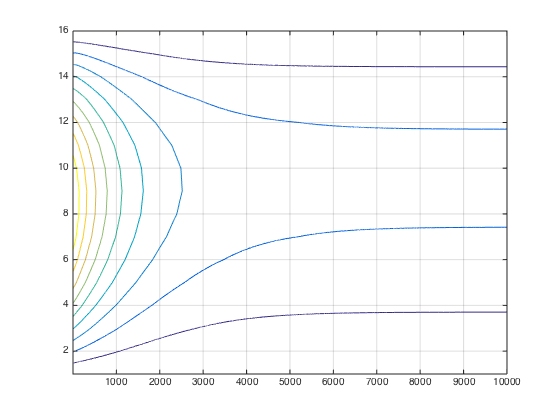
\includegraphics[width=\textwidth]{estimado_arriba}
                \caption{Estimado}
                \label{fig:gull}
        \end{subfigure}
        ~
        \begin{subfigure}[h]{0.45\textwidth}
                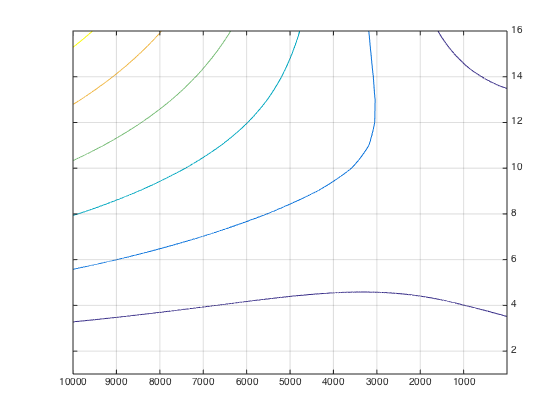
\includegraphics[width=\textwidth]{real_arriba}
                \caption{Real}
                \label{fig:tiger}
        \end{subfigure}
\end{figure}

Aquí podemos apreciar claramente, que la estimación mediante diferencias finitas se asemeja a la solución real. Si bien, no son exactamente iguales, el comportamiento es bastante similar.

\newpage
\subsection{Lineas de contorno: vista lateral}
\begin{figure}[!h]
        \centering
        \begin{subfigure}[h]{0.45\textwidth}
                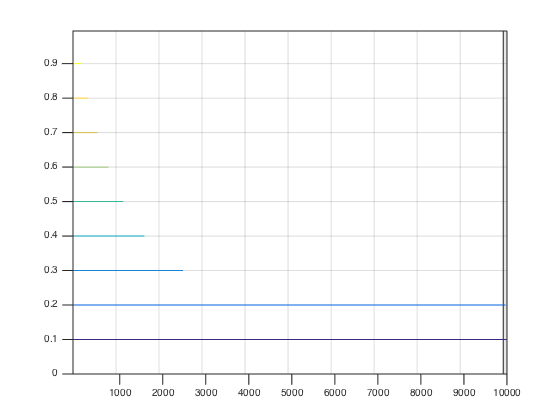
\includegraphics[width=\textwidth]{estimado_lateral}
                \caption{Estimado}
                \label{fig:gull}
        \end{subfigure}
        ~
        \begin{subfigure}[h]{0.45\textwidth}
                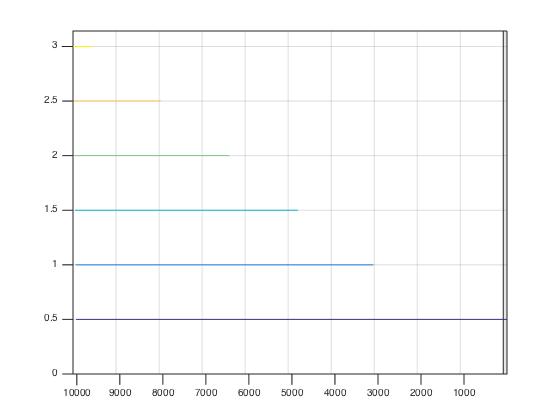
\includegraphics[width=\textwidth]{real_lateral}
                \caption{Real}
                \label{fig:tiger}
        \end{subfigure}
\end{figure}

\subsection{Lineas de contorno: vista diagonal}
\begin{figure}[!h]
        \centering
        \begin{subfigure}[h]{0.45\textwidth}
                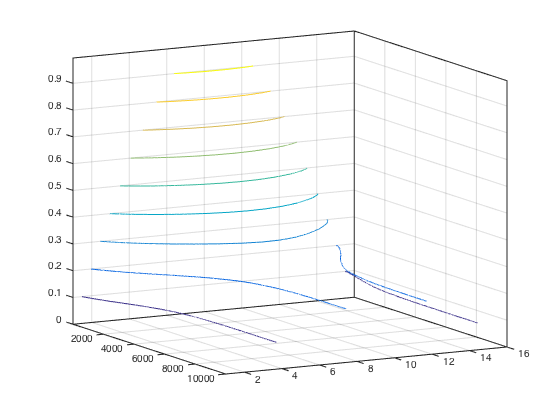
\includegraphics[width=\textwidth]{estimado_diagonal}
                \caption{Estimado}
                \label{fig:gull}
        \end{subfigure}
        ~
        \begin{subfigure}[h]{0.45\textwidth}
                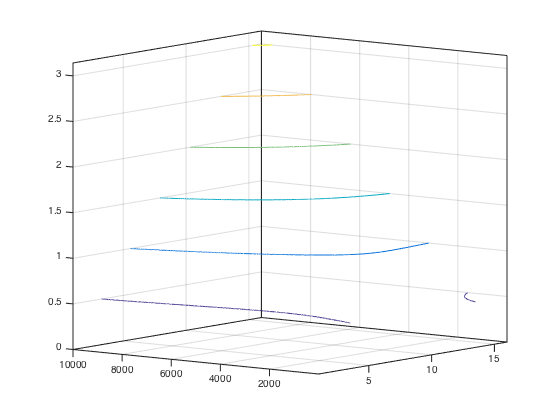
\includegraphics[width=\textwidth]{real_diagonal}
                \caption{Real}
                \label{fig:tiger}
        \end{subfigure}
\end{figure}

Por lo tanto, podemos apreciar gráficamente, que la estimación mediante diferencias finitas es una herramienta muy útil, que permite encontrar rapidamente estimaciones de funciones que pueden ser complejas de encontrar en primera instancia.

Las diferencias (error matemático), es una de las grandes desventajas de este método, el cual se arrastra y puede ser incremental, y es por eso que el parámetro $\lambda$ debe ser menor a 1, para asegurar que el problema se comporte de manera \textit{estable} (aunque esto no asegura que el problema converja totalmente).


\end{document} 